% --- ΚΕΦΑΛΑΙΟ 2: ΑΝΑΛΥΣΗ ΑΠΑΙΤΗΣΕΩΝ ---
\section{Ανάλυση Απαιτήσεων}
\label{sec:analysi_apaitiseon}
Το παρόν κεφάλαιο περιγράφει τις απαιτήσεις που τέθηκαν για την ανάπτυξη του εκπαιδευτικού λογισμικού εκμάθησης \eng{JavaScript}. Οι απαιτήσεις διακρίνονται σε λειτουργικές, οι οποίες καθορίζουν τις συγκεκριμένες ενέργειες και λειτουργίες που εκτελεί το σύστημα, και σε μη λειτουργικές, οι οποίες περιγράφουν τα ποιοτικά χαρακτηριστικά και τους περιορισμούς του συστήματος.

\subsection{Λειτουργικές Απαιτήσεις}
\label{sec:leitourgikes_apaitiseis}
Οι λειτουργικές απαιτήσεις καθορίζουν τις συγκεκριμένες υπηρεσίες και λειτουργίες που παρέχει η εφαρμογή στους χρήστες της.

\subsubsection{Ενότητες Διδασκαλίας}
\label{sec:enotites_didaskalias}
Η εφαρμογή πρέπει να παρέχει δομημένο εκπαιδευτικό περιεχόμενο για τη γλώσσα \eng{JavaScript}, οργανωμένο σε διακριτές εκπαιδευτικές ενότητες (\eng{Courses}) και επιμέρους μαθήματα (\eng{Lessons}). Συγκεκριμένα:
\begin{itemize}[leftmargin=*, noitemsep]
    \item \textbf{Παροχή Πολλαπλών Ενοτήτων (\eng{Courses}):} Το σύστημα προσφέρει τις ενότητες: "\eng{JavaScript Fundamentals}", "\eng{Intermediate Web Development with JS}", και "\eng{Advanced JavaScript \& Node.js}".
        \begin{figure}[h!]
          \centering
          
\includegraphics[scale=0.5]{images/courses_list.png}
          \caption{Λίστα διαθέσιμων κύκλων μαθημάτων.}
          \label{fig:courses_list_placeholder}
        \end{figure}
    \item \textbf{Δομή Ενοτήτων:} Κάθε \eng{Course} αποτελείται από υποενότητες (\eng{Modules}), οι οποίες περιέχουν τα μαθήματα (\eng{Lessons}).
        \begin{figure}[h!]
          \centering
          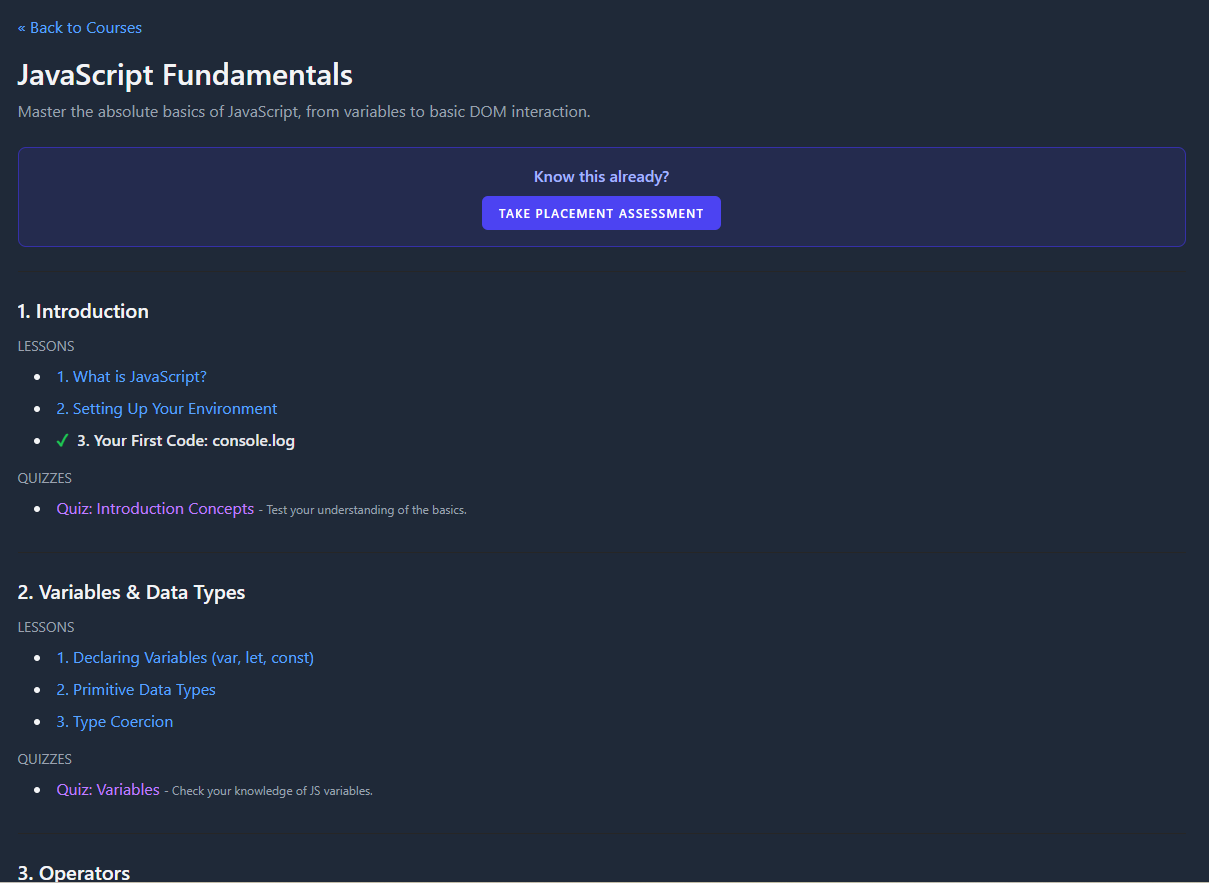
\includegraphics[scale=0.4]{images/module_example.png}
          \caption{Επισκόπηση ενός κύκλου μαθημάτων και των ενοτήτων του.}
          \label{fig:course_show_placeholder}
        \end{figure}
    \item \textbf{Περιεχόμενο Μαθημάτων (\eng{Lessons}):} Κάθε \eng{Lesson} περιλαμβάνει θεωρητικό υλικό, παραδείγματα κώδικα, και προαιρετικά οπτικοακουστικό υλικό (\eng{video\_embed\_html}).
        \begin{figure}[h!]
          \centering
          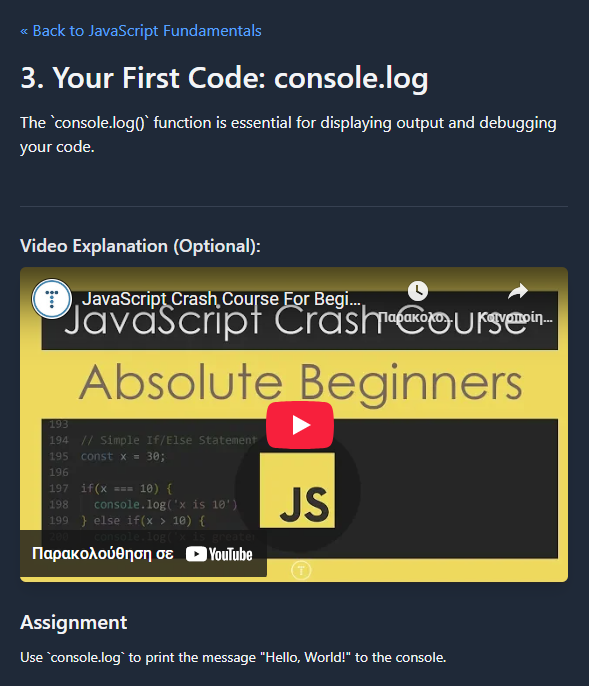
\includegraphics[scale=0.4]{images/lesson_content.png}
          \caption{Περιεχόμενο ενός μαθήματος.}
          \label{fig:lesson_content_placeholder}
        \end{figure}
    \item \textbf{Διαδραστικός Επεξεργαστής Κώδικα:} Κάθε \eng{Lesson} με άσκηση διαθέτει ενσωματωμένο \eng{code editor} (\eng{Monaco Editor}) για γραφή, τροποποίηση και \eng{client-side} εκτέλεση κώδικα.
    \item \textbf{Ασκήσεις Μαθημάτων:} Τα \eng{Lessons} μπορούν να περιλαμβάνουν \eng{assignment}. Η επιτυχής ολοκλήρωση (βάσει \eng{expected\_output}) μαρκάρει το μάθημα ως ολοκληρωμένο.
        \begin{figure}[h!]
          \centering
          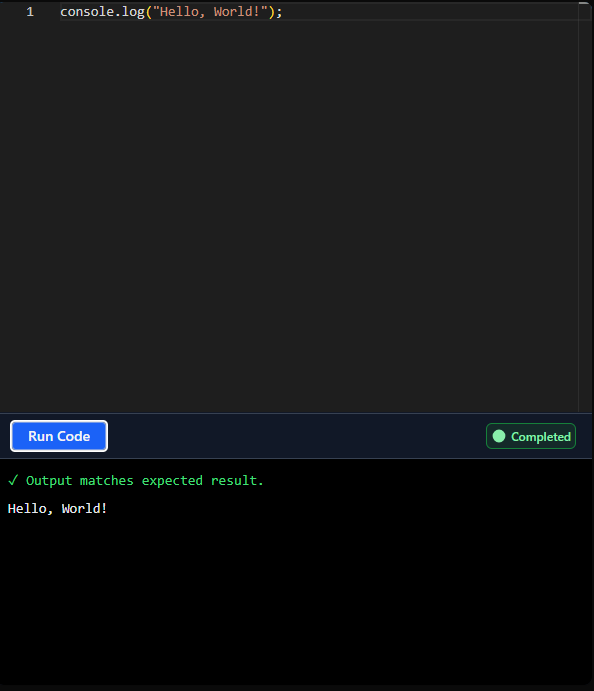
\includegraphics[scale=0.4]{images/lesson_editor.png}
          \caption{Διαδραστικός επεξεργαστής κώδικα και άσκηση μαθήματος.}
          \label{fig:lesson_editor_placeholder}
        \end{figure}
\end{itemize}

\subsubsection{Ερωτήσεις / Τεστ Αυτοαξιολόγησης}
\label{sec:test_autoaxiologisis}
Η εφαρμογή παρέχει σύστημα για \eng{quizzes} αυτοαξιολόγησης:
\begin{itemize}[leftmargin=*, noitemsep]
    \item \textbf{Τεστ ανά Ενότητα (\eng{Module Quizzes}):} Κάθε διδακτική υποενότητα (\eng{Module}) ενός \eng{Course} πρέπει να μπορεί να συνδέεται με ένα ή περισσότερα \eng{quizzes} που καλύπτουν το υλικό της συγκεκριμένης υποενότητας. Αυτά τα \eng{quizzes} βοηθούν τον χρήστη να ελέγξει την κατανόηση των εννοιών που μόλις διδάχθηκε.
    \item \textbf{Επαναληπτικά Τεστ:} Η εφαρμογή πρέπει να υποστηρίζει επαναληπτικά τεστ που συνδυάζουν ερωτήσεις από προηγούμενες ενότητες ή καλύπτουν το σύνολο ενός \eng{Course}. Συγκεκριμένα, υλοποιήθηκαν:
    \begin{itemize}[leftmargin=*, noitemsep]
        \item \textbf{Τελικό Επαναληπτικό \eng{Quiz} Κύκλου Μαθημάτων (\eng{Post-course Review Quiz}):} Στο τέλος κάθε \eng{Course}, ο χρήστης μπορεί να κάνει ένα επαναληπτικό \eng{quiz}. Αυτό το \eng{quiz} περιλαμβάνει δυναμικά ερωτήσεις στις οποίες ο χρήστης είχε απαντήσει λανθασμένα σε προηγούμενα \eng{module quizzes} του συγκεκριμένου \eng{course}, καθώς και τυχαίες νέες ερωτήσεις από το σύνολο του \eng{course}, για την ενίσχυση της μνήμης και της συνολικής κατανόησης.
        \item \textbf{Τυχαίο \eng{Quiz} Επανάληψης (\eng{Random Review Quiz}):} Τυχαίες ερωτήσεις από ολοκληρωμένα μαθήματα.
    \end{itemize}
    \item \textbf{Αξιολόγηση Αρχικού Επιπέδου (\eng{Pre-course Assessment Quiz}):} Για πρόταση σημείου εκκίνησης.
    \item \textbf{Ποικιλία Μορφών Ερωτήσεων:} Πολλαπλής Επιλογής, Σωστού/Λάθους, Συμπλήρωσης Κενού.
        \begin{figure}[h!]
          \centering
          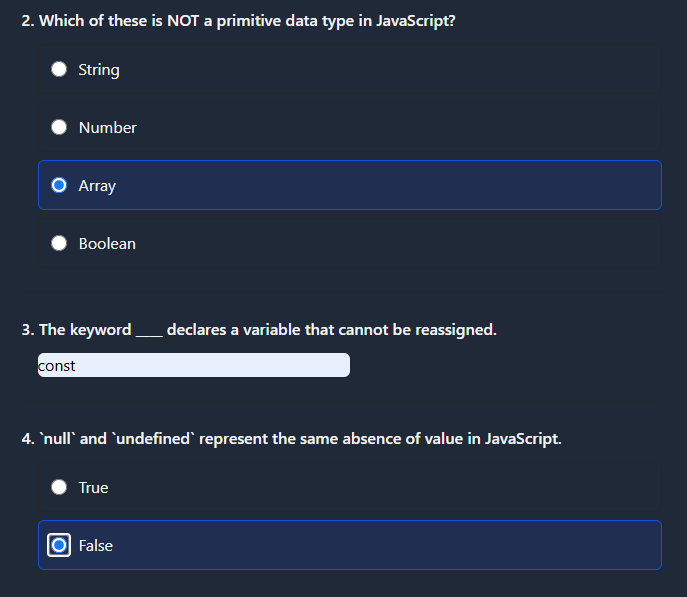
\includegraphics[scale=0.4]{images/question_types.png}
          \caption{Διεπαφή διεξαγωγής \eng{Quiz}.}
          \label{fig:quiz_interface_placeholder}
        \end{figure}
    \item \textbf{Διεπαφή Διεξαγωγής \eng{Quiz}:} Φιλικό περιβάλλον, άμεση ανατροφοδότηση (σκορ, σωστές/λανθασμένες απαντήσεις, εξηγήσεις).
    \item \textbf{Συστάσεις Βάσει Αποτελεσμάτων:} Πρόταση επανάληψης μαθημάτων και εξωτερικών πηγών.
        \begin{figure}[h!]
          \centering
          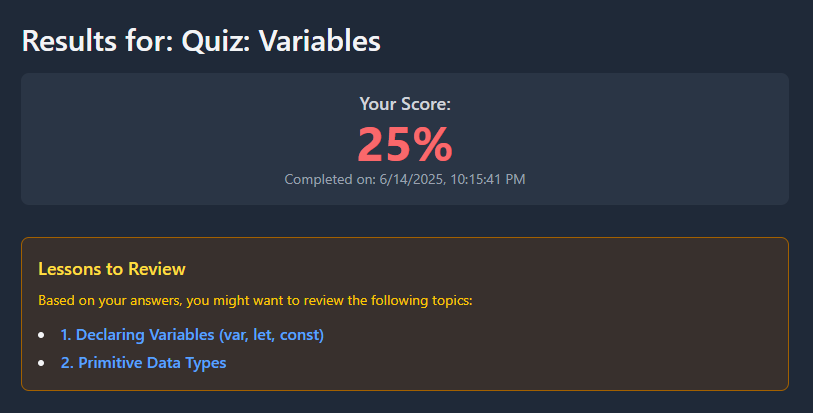
\includegraphics[scale=0.4]{images/quiz_results_recommendations.png}
          \caption{Αποτελέσματα \eng{Quiz} και προτάσεις επανάληψης.}
          \label{fig:quiz_results_placeholder}
        \end{figure}
\end{itemize}

\subsubsection{Αποθήκευση Στατιστικών Προόδου}
\label{sec:statistika_proodou}
Η εφαρμογή καταγράφει και αποθηκεύει δεδομένα προόδου:
\begin{itemize}[leftmargin=*, noitemsep]
    \item \textbf{Ολοκλήρωση Μαθημάτων (\eng{Lessons}):} Μέσω του πίνακα \eng{user\_progress} (\eng{user\_id, lesson\_id, completed\_at}).
    \item \textbf{Προσπάθειες και Αποτελέσματα \eng{Quiz}:} Στους πίνακες \eng{quiz\_attempts} (\eng{user\_id, quiz\_id (nullable), type, score, timestamps}) και \eng{quiz\_answers} (\eng{attempt\_id, question\_id, user\_answer, is\_correct}).
    \item \textbf{Δεδομένα Προφίλ και Προτιμήσεων Χρήστη:} Στον πίνακα \eng{users}.
\end{itemize}

\subsubsection{Προσαρμοσμένη Μάθηση (\eng{Adaptive Learning})}
\label{sec:adaptive_learning}
Η εφαρμογή στοχεύει στην παροχή μιας εμπειρίας προσαρμοσμένης μάθησης, όπου το εκπαιδευτικό περιεχόμενο και οι δραστηριότητες προσαρμόζονται δυναμικά στις επιδόσεις, τις προτιμήσεις και τις ανάγκες του κάθε μαθητή. Αυτό επιτυγχάνεται μέσω των παρακάτω μηχανισμών:
\begin{itemize}[leftmargin=*, noitemsep]
    \item \textbf{Αξιολόγηση Αρχικού Επιπέδου και Πρόταση Διαδρομής:} Μέσω του \eng{Pre-course Assessment Quiz} και του \eng{CourseAssessmentController}. Πριν την έναρξη ενός κύκλου μαθημάτων (\eng{Course}), ο χρήστης έχει τη δυνατότητα να συμμετάσχει σε ένα quiz αξιολόγησης αρχικού επιπέδου (\eng{Pre-course Assessment Quiz}). Βάσει των απαντήσεών του σε αυτό το \eng{quiz}, το σύστημα αξιολογεί την κατανόησή του σε θέματα που καλύπτονται στα αρχικά μαθήματα του \eng{course}. Εάν ο χρήστης επιδείξει επαρκή γνώση σε συγκεκριμένες ενότητες, η εφαρμογή του προτείνει να παρακάμψει τα αντίστοιχα αρχικά μαθήματα και να ξεκινήσει από ένα πιο προχωρημένο σημείο, αποφεύγοντας την επανάληψη υλικού που ήδη κατέχει.
        \begin{figure}[h!]
          \centering
          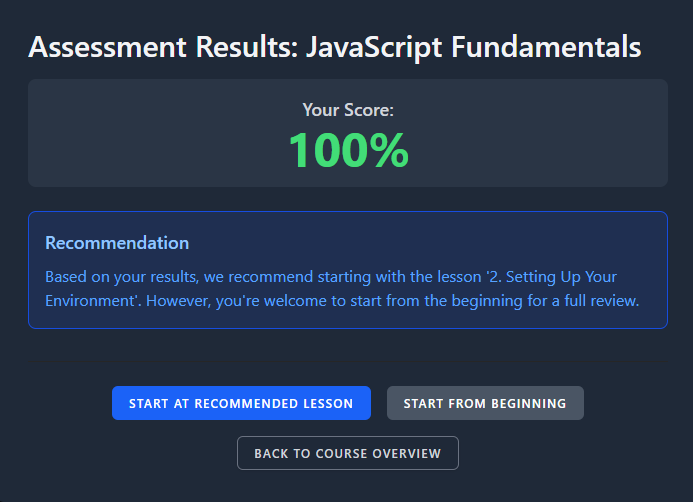
\includegraphics[scale=0.5]{images/assessment_result.png}
          \caption{Πρόταση μαθήματος μετά από αξιολόγηση αρχικού επιπέδου.}
          \label{fig:pre_course_result_placeholder}
        \end{figure}
    \item \textbf{Στοχευμένη Επανάληψη και Ενισχυτικό Υλικό:} Μέσω του \eng{Post-course Review Quiz}, του \eng{CourseReviewController} και του πίνακα \eng{external\_resources}.Μετά την ολοκλήρωση ενός τελικού επαναληπτικού \eng{quiz} ενός \eng{course} (\eng{Post-course Review Quiz}), εάν ο χρήστης εξακολουθεί να κάνει λάθη σε ερωτήσεις που αντιστοιχούν σε συγκεκριμένα μαθήματα, το σύστημα: Τον ανακατευθύνει ή του προτείνει να επισκεφθεί ξανά τα μαθήματα (\eng{lessons}) στα οποία παρουσίασε αδυναμίες. Παρέχει συνδέσμους προς επιλεγμένες εξωτερικές πηγές υλικού (π.χ. άρθρα, βίντεο, τεκμηρίωση) σχετικές με τα συγκεκριμένα μαθήματα, για περαιτέρω μελέτη και ενίσχυση της κατανόησης.
    \item \textbf{Προσαρμογή Παρουσίασης Περιεχομένου βάσει Μαθησιακού Στυλ:} Ο χρήστης μπορεί να δηλώσει στο \eng{dashboard} τον προτιμώμενο τρόπο μάθησης (π.χ. '\eng{visual}' για έμφαση σε οπτικό υλικό, '\eng{reading}' για έμφαση σε κείμενο). Στα μαθήματα που διαθέτουν τόσο κειμενικό όσο και οπτικοακουστικό υλικό (π.χ. ενσωματωμένα βίντεο), η εφαρμογή προσαρμόζει τη σειρά εμφάνισης αυτών των στοιχείων. Για παράδειγμα, ένας χρήστης που προτιμά οπτικό υλικό θα δει πρώτα το βίντεο και μετά το σχετικό κείμενο.
        \begin{figure}[h!]
          \centering
          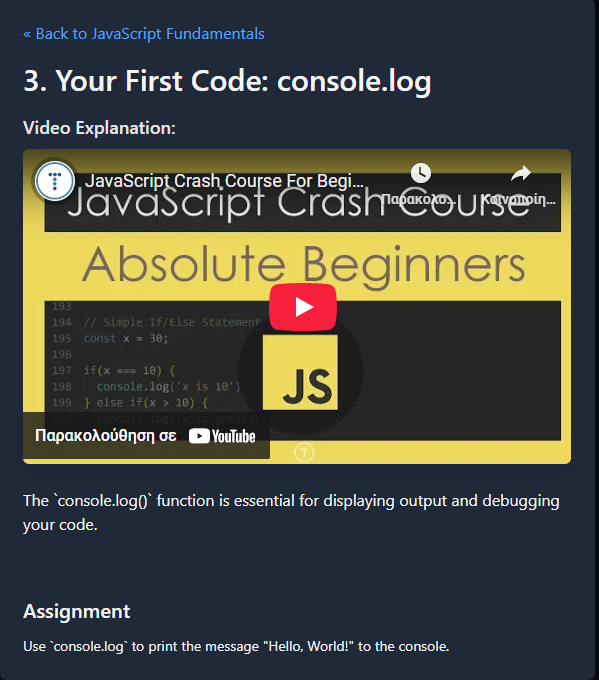
\includegraphics[scale=0.5]{images/visual_learner_lesson.png}
          \caption{Προσαρμογή εμφάνισης περιεχομένου βάσει μαθησιακού στυλ.}
          \label{fig:lesson_visual_placeholder}
        \end{figure}
    \item \textbf{Καθοδηγούμενα Μονοπάτια Μάθησης (\eng{Learning Paths}):} Ο χρήστης μπορεί να επιλέξει μια προκαθορισμένη μαθησιακή διαδρομή (\eng{Learning Path}) που αντιστοιχεί σε συγκεκριμένους εκπαιδευτικούς ή επαγγελματικούς στόχους (π.χ. \eng{"Frontend Developer Path", "Backend JavaScript Developer Path"}). Η εφαρμογή, βάσει της επιλεγμένης διαδρομής και της προόδου του χρήστη στα courses που την αποτελούν, προτείνει το επόμενο λογικό \eng{course} ή μάθημα για παρακολούθηση, παρέχοντας μια πιο δομημένη και καθοδηγούμενη πορεία μάθησης.
        \begin{figure}[h!]
          \centering
          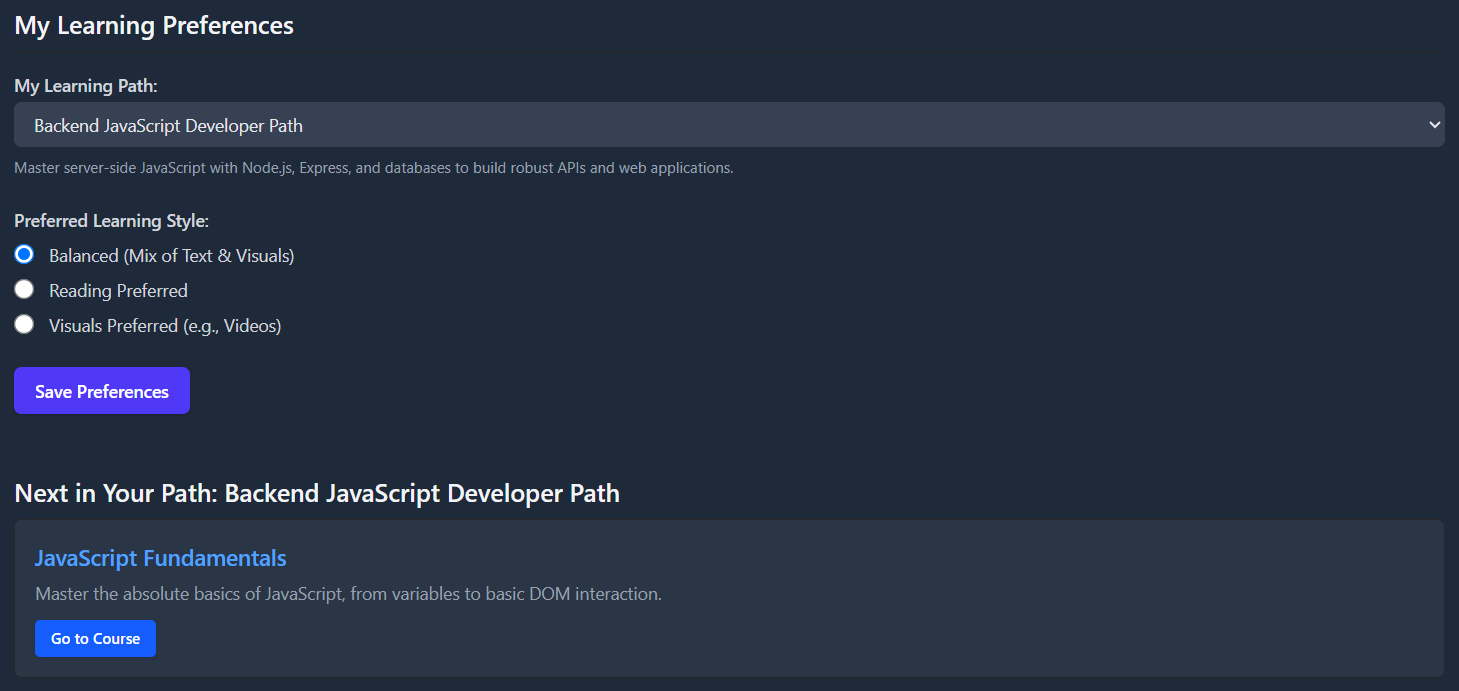
\includegraphics[scale=0.4]{learning_path.png}
          \caption{Επιλεγμένη μαθησιακή διαδρομή και προτεινόμενο επόμενο μάθημα.}
          \label{fig:dashboard_path_placeholder}
        \end{figure}
    \item \textbf{Ρύθμιση Δυσκολίας Ασκήσεων/\eng{Quiz}:} Αν και δεν έχει υλοποιηθεί πλήρως δυναμική ρύθμιση δυσκολίας εντός ενός \eng{quiz}, η επιλογή των ερωτήσεων στα επαναληπτικά \eng{quizzes} (\eng{Post-course Review} και \eng{Random Review}) λαμβάνει υπόψη τις προηγούμενες επιδόσεις (εστιάζοντας σε λανθασμένες απαντήσεις), προσφέροντας έμμεσα μια μορφή προσαρμογής της δυσκολίας στην επανάληψη.
\end{itemize}

\subsubsection{Διαχείριση Χρήστη}
\label{sec:diacheirisi_xristi}
Παρέχονται βασικές λειτουργίες διαχείρισης λογαριασμού:
\begin{itemize}[leftmargin=*, noitemsep]
    \item Εγγραφή, Σύνδεση, Αποσύνδεση.
    \item Επεξεργασία Προφίλ (όνομα, \eng{email}, \eng{password}) και Μαθησιακών Προτιμήσεων (στυλ, \eng{path}) μέσω του \eng{Dashboard} και του \eng{UserPreferenceController}.
        \begin{figure}[h!]
          \centering
          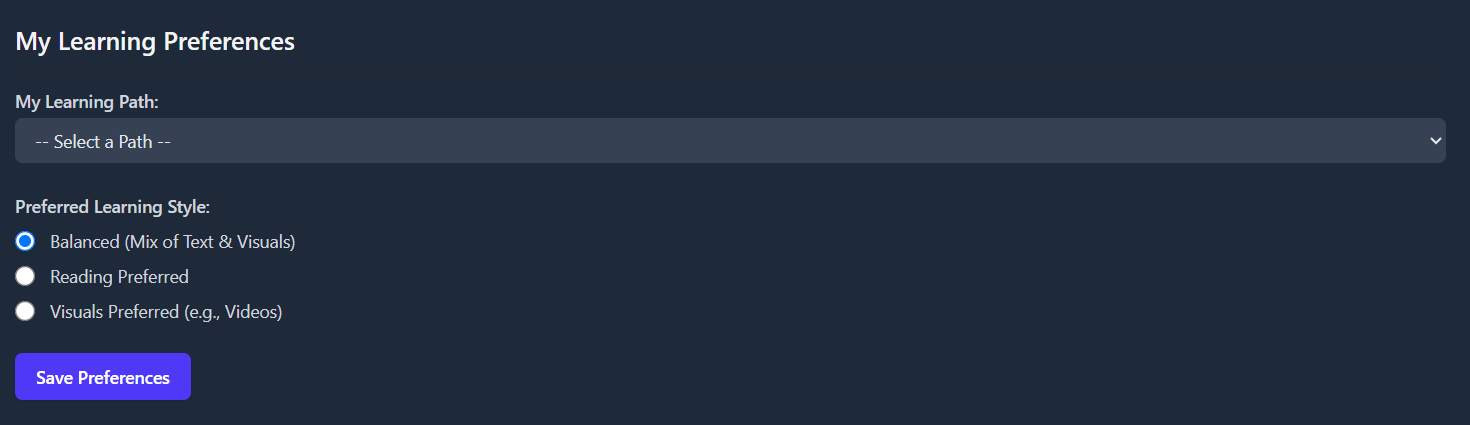
\includegraphics[scale=0.4]{preferences.png}
          \caption{Διαχείριση προτιμήσεων χρήστη στο \eng{Dashboard}.}
          \label{fig:dashboard_prefs_placeholder}
        \end{figure}
\end{itemize}

\subsubsection{Προβολή Αναφορών Προόδου}
\label{sec:anafores_proodou}
Οπτικοποιημένες αναφορές προόδου και στατιστικά στοιχεία:
\begin{itemize}[leftmargin=*, noitemsep]
    \item Μαθησιακό Σερί (\eng{Learning Streak}).
    \item Σύνολο Προσπαθειών σε \eng{Quiz}.
    \item Κατανομή Αποτελεσμάτων \eng{Quiz} (Πίτα).
    \item Γράφημα Ολοκληρωμένων Μαθημάτων ανά Ημέρα ("\eng{Contribution Graph}").
        \begin{figure}[h!]
          \centering
          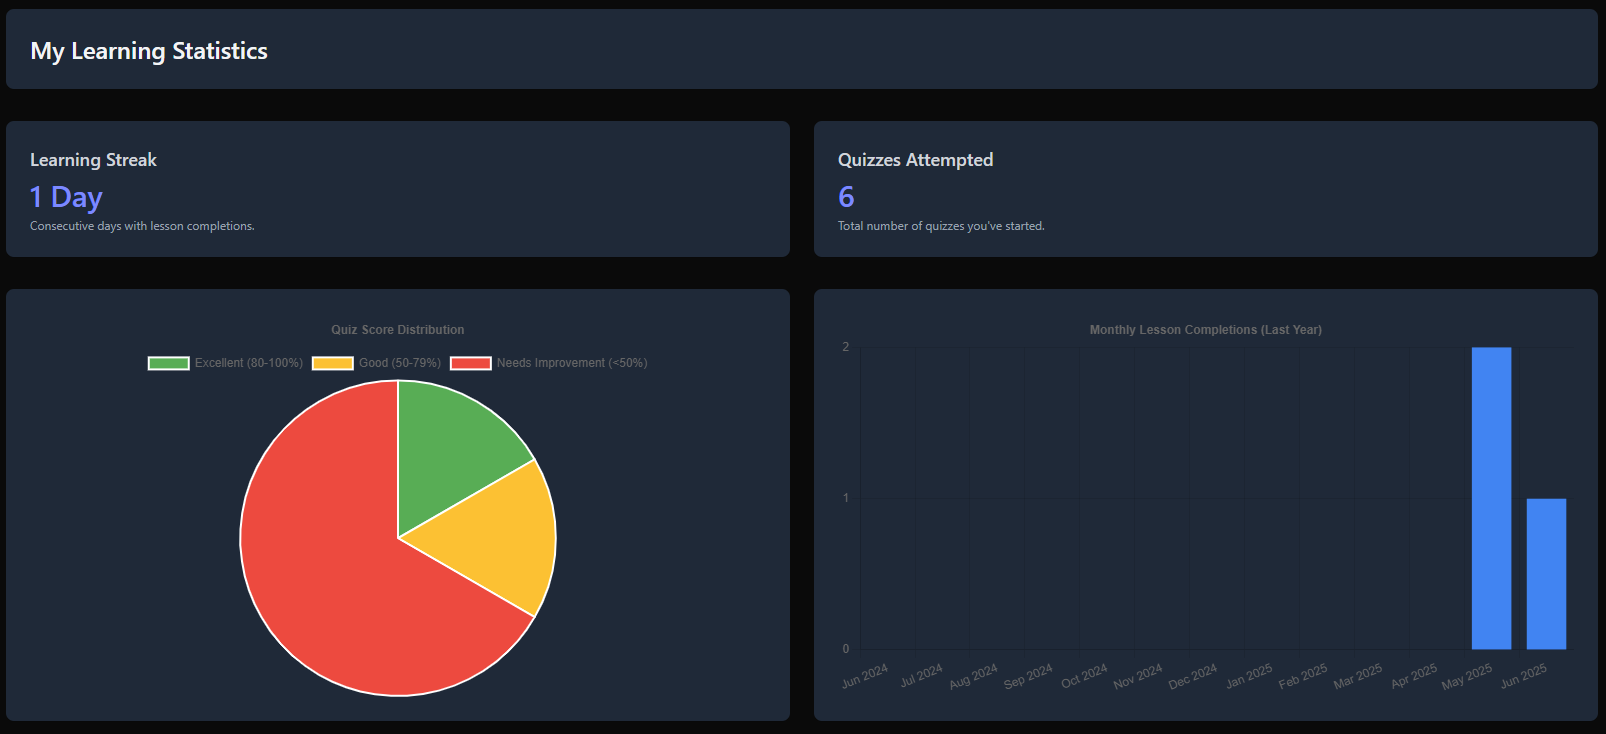
\includegraphics[scale=0.2]{statistics_page.png}
          \caption{Σελίδα στατιστικών προόδου χρήστη.}
          \label{fig:stats_page_placeholder}
        \end{figure}
\end{itemize}

\subsection{Μη Λειτουργικές Απαιτήσεις}
\label{sec:mi_leitourgikes_apaitiseis}
Πέραν των λειτουργιών, τέθηκαν και ποιοτικές απαιτήσεις:
\begin{itemize}[leftmargin=*, noitemsep]
    \item \textbf{Χρηστικότητα (\eng{Usability}):} Διαισθητικό και εύχρηστο περιβάλλον.
    \item \textbf{Απόδοση (\eng{Performance}):} Λογικοί χρόνοι φόρτωσης, άμεση απόκριση του \eng{editor}.
    \item \textbf{Ασφάλεια (\eng{Security}):} Προστασία δεδομένων χρήστη, \eng{client-side} εκτέλεση κώδικα από ελεγχόμενες πηγές περιεχομένου.
    \item \textbf{Συντηρησιμότητα (\eng{Maintainability}):} Οργανωμένος κώδικας.
    \item \textbf{Συμβατότητα (\eng{Compatibility}):} Λειτουργία σε σύγχρονους \eng{web browsers}.
\end{itemize}